\documentclass[landscape,a4paper]{article}

% Page setup
\usepackage[top=1mm,bottom=2mm,left=1mm,right=1mm]{geometry}
\usepackage{multicol}
\usepackage{microtype}

% Math packages
\usepackage{amsmath,amsfonts,amssymb,amsthm}
\usepackage{dsfont}

% Graphics and visual packages
\usepackage{graphicx}
\usepackage{float}
\usepackage{xcolor}
\usepackage{tikz}
\usetikzlibrary{shapes,positioning,arrows,fit,calc,graphs,graphs.standard}
\usepackage{fancybox}
\usepackage{array}

% Code and algorithm packages
\usepackage{algorithm,algorithmic}
\usepackage{capt-of}
\usepackage{listings}

% Document utilities
\usepackage{pdfpages}

% Formatting and styling packages
\usepackage{titlesec}
\usepackage{enumitem}
\usepackage{helvet}

% Font settings
\renewcommand{\familydefault}{\sfdefault}

% Document formatting settings
\setcounter{secnumdepth}{0} % No section numbering
\setlength{\fboxsep}{1pt} % Color box padding

% Title formatting
\titleformat{\section}{\fontsize{7.2pt}{7.2pt}\selectfont\bfseries}{\thesection}{0em}{\colorbox{yellow!70}}
\titleformat{\subsection}{\fontsize{6pt}{6pt}\selectfont\bfseries}{\thesubsection}{0em}{\colorbox{green!20}}
\titleformat{\subsubsection}{\fontsize{6pt}{6pt}\selectfont\bfseries}{\thesubsubsection}{0em}{\colorbox{blue!10}}
\titlespacing{\section}{0pt}{0pt}{0pt}
\titlespacing{\subsection}{0pt}{0pt}{0pt}
\titlespacing{\subsubsection}{0pt}{0pt}{0pt}

% Math symbols and spacing
\renewcommand{\vdots}{\mathrel{\raisebox{0pt}{.}\kern-1.4pt\raisebox{1.2pt}{.}\kern-1.4pt\raisebox{2.4pt}{.}}}
\renewcommand{\cdots}{\mathrel{\cdot\kern-2pt\cdot\kern-2pt\cdot}}

% Macros
\newcommand{\todo}{\textbf{\textcolor{red}{TODO }}}
\newcommand{\revisit}{\textbf{\textcolor{orange}{REVISIT }}}

\begin{document}

% Grayed out text environment
\newenvironment{graytext}{\color{gray}\ignorespaces}{}

% Document settings
\raggedright
\fontsize{6pt}{6.2pt}\selectfont

% Global indentation variables
\newlength{\listindentone}
\newlength{\listindenttwo}
\setlength{\listindentone}{10pt}
\setlength{\listindenttwo}{4pt}

% List spacing control
\setlist[itemize,1]{nosep,leftmargin=\listindentone}
\setlist[enumerate,1]{nosep,leftmargin=\listindentone}
\setlist[itemize,2]{nosep,leftmargin=\listindenttwo}
\setlist[enumerate,2]{nosep,leftmargin=\listindenttwo}

% Math environment spacing control
\setlength{\abovedisplayskip}{0.5pt}
\setlength{\belowdisplayskip}{0.5pt}
\setlength{\abovedisplayshortskip}{1pt}
\setlength{\belowdisplayshortskip}{1pt}
\setlength{\arraycolsep}{0.5pt}
\setlength{\jot}{1pt}

% Table spacing control
\setlength{\abovecaptionskip}{1pt}
\setlength{\belowcaptionskip}{1pt}
\setlength{\intextsep}{1pt}

% Center environment spacing control
\setlength{\topsep}{1pt}
\setlength{\partopsep}{0pt}

% Multi-column layout
\begin{multicols*}{4}
    \columnseprule=0.2pt

    % Content sections
    \section{General Concepts}
\subsection{General Terms}
\begin{itemize}
    \item \textbf{Latency:} Time taken for a packet to travel from source to destination.
    \item \textbf{Throughput:} Rate of successful message delivery over a communication channel.
    \item \textbf{Bandwidth:} Maximum rate of data transfer across a given path.
    \item \textbf{Jitter:} Variation in packet arrival time.
    \item \textbf{Reliability:} Ability of a system to function under stated conditions for a specified period.
\end{itemize}

\subsection{Mathematical Foundations}
\subsubsection{Probability}

\subsection{Computer networks vs Distributed systems}
\subsubsection{Circuit and Packet Switching}
\subsubsection{Timing}
\subsubsection{Multiplexing}

\subsection{The OSI Model}
\begin{itemize}
    \item \textbf{Layers (5):} Physical, (Data) Link, (Inter)Network, Transport, Application.
    \item \textbf{Physical:} Move bits on a link (signals, timing, encoding).
    \item \textbf{Link:} Frames on local network, MAC addressing, error detection.
    \item \textbf{Network:} Packet delivery across networks, routing (IP).
    \item \textbf{Transport:} End-to-end process communication, reliability/flow control (TCP/UDP).
    \item \textbf{Application:} End-user services/protocols (HTTP, SMTP, DNS, etc.).
\end{itemize}

    \section{Link Layer \& Local Area Networks (LAN)}
\subsection{Shared Medium Intuition}
\begin{itemize}
	\item Nodes broadcast on same channel; only one can transmit at a time.
	\item Simultaneous transmit $\Rightarrow$ collision $\Rightarrow$ data lost.
	\item Sender uses full link bandwidth while transmitting.
\end{itemize}

\subsection{Definitions}
\begin{itemize}
	\item \textbf{Bandwidth:} max data rate of channel ($B$).
	\item \textbf{Throughput:} fraction of bandwidth used to send traffic.
	\item \textbf{Goodput:} fraction of bandwidth used for successful data.
	\item $\eta=\frac{\text{avg effective bandwidth}}{\text{total bandwidth}}=\frac{\text{avg effective time}}{\text{total time}}$, $0\le\eta\le1$.
\end{itemize}

\subsection{Multiple Access Domains}
\begin{itemize}
    \item \textbf{Multiple Access Domain:} set of nodes sharing a common channel.
    \item \textbf{Channel Partitioning:} divide channel into smaller "pieces" (time/freq/code).
    \item \textbf{Random Access:} transmit at will; handle collisions (ALOHA, CSMA).
    \item \textbf{Taking Turns:} nodes take turns to transmit (polling/token passing).
\end{itemize}
\subsection{ALOHA protocol}
\begin{itemize}
	\item Random access on shared medium; collisions if overlap. Frame time $T$ (size $L$, rate $B$): $T=L/B$.
	\item \textbf{Binomial model:} $N$ users, each transmits in a slot w.p. $p$.
	\item \textbf{Poisson model:} aggregate attempts are Poisson with rate $G$ (attempts/slot).
	\item \textbf{Slotted ALOHA (align to slots):}
	\begin{itemize}
		\item Success if exactly one tx in a slot.
		\item Binomial: $P(\text{succ})=Np(1-p)^{N-1}$, max at $p=1/N$ gives $S_{\max}\approx 1/e$.
		\item Poisson: $S=Ge^{-G}$, $S_{\max}=1/e$ at $G=1$.
	\end{itemize}
	\item \textbf{Pure ALOHA (no slots):}
	\begin{itemize}
		\item Vulnerable period $2T$.
		\item Binomial (approx): $P(\text{succ})\approx Np(1-p)^{2(N-1)}$, max at $p\approx 1/(2N)$ gives $S_{\max}\approx 1/(2e)$.
		\item Poisson: $S=Ge^{-2G}$, $S_{\max}=1/(2e)$ at $G=1/2$.
	\end{itemize}
\end{itemize}

\subsection{CSMA (Carrier Sense Multiple Access)}
\begin{itemize}
    \item Listen before tx; if channel idle, transmit entire frame; else wait.
    \item \textbf{Propagation delay} $\tau$: time for signal to propagate between 2 farthest nodes.
    \item \textbf{CSMA/CD (Collision Detection):} abort tx on collision detection; reduces wasted time.
    \item \textbf{CSMA/CD efficiency:} $\eta=\frac{1}{1+5\frac{d_{\text{prop}}}{d_{\text{trans}}}}$.
\end{itemize}

\subsubsection{CSMA/CD (Collision Detection)}
\begin{itemize}
	\item Detect collisions while transmitting; send jam; then backoff and retry.
	\item \textbf{Binary exponential backoff:} after $m$-th collision pick $k\in\{0,\ldots,2^m-1\}$, wait $k$ slots.
\end{itemize}
\subsubsection{CSMA/CA (Collision Avoidance)}
\begin{itemize}
	\item Used in Wi-Fi: cannot detect collisions reliably, so avoid them.
	\item If channel idle, wait DIFS then transmit; if busy, pick random backoff slots.
	\item Receiver replies with ACK after SIFS; missing ACK implies collision.
\end{itemize}
\subsubsection{CSMA persistence}
\begin{itemize}
	\item \textbf{1-persistent:} transmit immediately when channel becomes idle (high collision under load).
	\item \textbf{0-persistent:} wait random backoff after busy (lower collision, higher delay).
	\item \textbf{$p$-persistent:} when idle, transmit with prob. $p$ each slot (tradeoff).
\end{itemize}

\subsection{Single (Logical) Link in practice}
\subsubsection{MAC Addresses}
\begin{itemize}
	\item Link-layer address unique per NIC (Network Interface Card); assigned by IEEE OUI.
	\item Used to deliver frames on same LAN; flat (non-hierarchical), portable across LANs.
	\item Usually burned-in, but can be software-set.
\end{itemize}
\subsubsection{Ethernet}
\begin{itemize}
	\item Dominant wired LAN; many speed generations; cheap NICs.
	\item \textbf{CSMA/CD (classic shared medium):}
	\begin{enumerate}
		\item Sense channel; if idle transmit, else wait.
		\item If collision detected while tx, abort and send jam.
		\item \textbf{Binary exponential backoff:} after $m$-th collision pick $k\in\{0,\ldots,2^m-1\}$, wait $k\cdot512$ bit-times, retry.
	\end{enumerate}
\end{itemize}

\subsection{Interconnecting broadcast domains}
\begin{itemize}
	\item \textbf{Switch:}
    \begin{itemize}
        \item link-layer device that breaks broadcast domains; stores/forwards frames using MAC table.
        \item Transparent to hosts; self-learning (no manual config), entries age out (TTL).
        \item Each link is its own collision domain; enables simultaneous transmissions.
        \item Forwarding: if dest known on incoming port $\Rightarrow$ drop; else forward to port; if unknown $\Rightarrow$ flood.
		\item \textbf{Switch table:} (MAC, port, TTL). Learn from source MAC+ingress port on each frame.
    \end{itemize}
    \item \textbf{Loops:} cause broadcast storms, multiple frame copies, MAC table instability.
	\item \textbf{Spanning Tree Protocol (STP):} disable links to eliminate loops; elect root, compute shortest-path tree.
	\item \textbf{HELLO/BPDU fields:} SID (switch ID), RID (root ID), DTR (distance to root).
	\item Root selection: prefer lower RID; then lower DTR; then lower SID (tie-break).
\end{itemize}

\subsection{Errors Detection}
\begin{itemize}
	\item Goal: detect (and sometimes correct) bit errors introduced by noise on the link.
	\item \textbf{Repetition code (3-repetition):} send each bit 3 times; majority vote corrects 1 error, detects up to 2.
	\item \textbf{1D parity:} add one parity bit so total 1s is even/odd; detects any odd number of bit errors, cannot locate/correct.
	\item \textbf{2D parity:} arrange bits in a matrix with row+column parity; detects many multi-bit errors and can correct a single-bit error (intersection).
	\item \textbf{CRC:} \todo \textbf{Consider removing this if not in Exams} treat bits as polynomial over $GF(2)$; append $r$-bit remainder so frame is divisible by generator $G(x)$.
	\item CRC detects all single-bit errors, all burst errors of length $\le r$, and most longer bursts (prob. of miss $\approx 2^{-r}$).
\end{itemize}

\section{"Layer 2.5" - ARP}
ARP is generally considered to be part of Layer 2 (Data Link Layer), but it works directly to support Layer 3 (Network Layer).
\begin{itemize}
    \item Why it's Layer 2: ARP messages are encapsulated directly into Ethernet frames. They do not have an IP header (Layer 3) and they cannot be routed outside of your local network (LAN).
    \item Why it feels like Layer 3: Its entire purpose is to handle Layer 3 information (IP addresses). It is the mechanism that allows Layer 3 to actually function on physical hardware.
\end{itemize}
\subsection{Address Resolution Protocol (ARP)}
\begin{itemize}
	\item Translates between MAC addresses and IP addresses on a LAN.
	\item Needed because Layer 3 provides the IP, but frames on Layer 2 need a destination MAC.
	\item To send outside the LAN, the packet uses the IP of the destination but the MAC of the next-hop router; routers then forward using their own L2 on each hop.
	\item Hosts use DHCP and routing to know whether the destination IP is on the same LAN or remote.
	\item Each node maintains an \textbf{ARP cache} (IP $\rightarrow$ MAC table).
	\item If the mapping is missing, send an \textbf{ARP request} (broadcast in the local broadcast domain).
	\item The target replies with an \textbf{ARP response} containing its MAC, which is stored in the cache.
	\item ARP messages stay within a single broadcast domain (not routed).
\end{itemize}
    \section{Network Layer (IP \& Routing)}

\subsection{Introduction to IP addressing}
\begin{itemize}
	\item IPv4 address = 32 bits (a.b.c.d), identifies interface (host/router can have multiple interfaces).
	\item Subnet vs host split via CIDR: a.b.c.d/$x$ where $x$ = prefix length (subnet mask).
	\item Example: 192.168.1.178/24 $\Rightarrow$ subnet 192.168.1, host 178.
	\item Hierarchical addressing enables routing scalability; ISPs advertise prefixes.
	\item Forwarding uses \textbf{longest prefix match}.
	\item \textbf{Address discovery protocols:}
\end{itemize}

\begin{center}
    \textbf{IP Packet Diagram}
    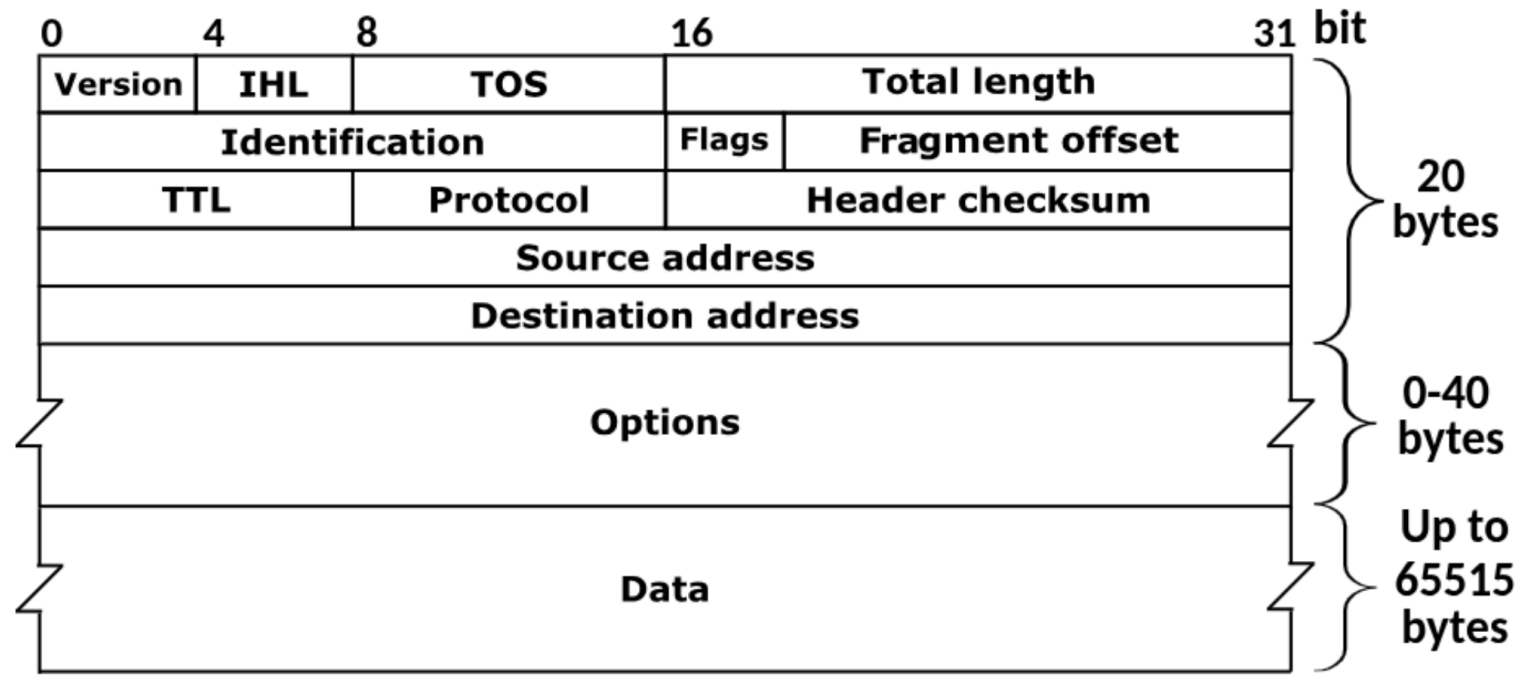
\includegraphics[width=0.9\columnwidth]{images/ip_packet_diagram.png}
\end{center}

    \section{Transport Layer (TCP \& UDP)}

\subsection{TCP (Transmission Control Protocol)}
\begin{itemize}
    \item Reliable, in-order byte stream; receiver ACKs received data.
    \item \textbf{vs. UDP:} UDP provides port+IP multiplexing (best effort) with no reliability, ordering, or flow control.
    \item \textbf{Sequence \#:} The byte number of the \textit{first} byte of data in the segment.
    \item \textbf{ACK \#:} The \textit{next expected} byte (Cumulative ACK).
    \item \textbf{MTU vs. MSS:}
    \begin{itemize}
        \item \textbf{MTU:} Max Transfer Unit (max packet size on link, e.g., 1500B).
        \item \textbf{MSS:} Max Segment Size (max payload). $MSS = MTU - (IP_{Header} + TCP_{Header})$. \\ Typically $MSS = MTU - 40$ (so $MSS < MTU$).
    \end{itemize}
	\item \textbf{TCP header (min 20B, + options):} src/dst ports, Seq \#, ACK \#, flags (SYN/ACK/FIN/RST/PSH/URG), window, checksum, urgent pointer.
\end{itemize}

\subsubsection{Connection Setup (3-Way Handshake)}
\begin{enumerate}
	\item Client $\to$ Server: \textbf{SYN}, Seq $= x$.\\
	\quad Announces client ISN (Initial Sequence Number, $x$) and requests connection.
	\item Server $\to$ Client: \textbf{SYN + ACK}, Seq $= y$, ACK $= x+1$.\\
	\quad Accepts, advertises server ISN, and ACKs client ISN.
	\item Client $\to$ Server: \textbf{ACK}, Seq $= x+1$, ACK $= y+1$.\\
	\quad Final ACK; both sides synchronized.
    \item (Connection Established)
\end{enumerate}

\subsubsection{Connection Teardown}
\begin{enumerate}
    \item Client sends \textbf{FIN}.
    \item Server replies \textbf{ACK}. (Client enters FIN\_WAIT\_2).
    \item Server sends \textbf{FIN}.
    \item Client replies \textbf{ACK}, waits \textbf{TIME\_WAIT} (usually 2*MSL), then closes.
\end{enumerate}

\subsubsection{Reliable data transfer (sender)}
\begin{itemize}
	\item Maintain sequence number and buffer; segment and send data.
	\item Send while window allows: $lastByteSent - lastByteAcked \le RW$ (receiver window).
	\item Start timer if not running; on timeout, retransmit the oldest unACKed segment.
\end{itemize}

\subsubsection{Reliable data transfer (receiver)}
\begin{itemize}
	\item Deliver in-order data and send cumulative ACK.
	\item If out-of-order segment arrives, send ACK for last in-order byte (duplicate ACK).
\end{itemize}

\subsubsection{Retransmissions}
\begin{itemize}
	\item Retransmit on either \textbf{timeout} or \textbf{duplicate ACKs}.
	\item \textbf{Fast retransmit:} many duplicate ACKs imply loss before timeout.
\end{itemize}

\subsubsection{RTT estimation}
\begin{itemize}
	\item Goal: set timeout slightly above RTT to avoid premature retransmits but still react fast to loss.
	\item \textbf{SampleRTT:} time from sending a segment until its first ACK returns (ignore retransmitted samples).
	\item Now we can compute a smoothed RTT which is exponentially weighted moving average of recent samples:
	\[ \textbf{EstimatedRTT} \leftarrow (1-\alpha)\,\text{EstimatedRTT} + \alpha\,\text{SampleRTT}\]
	typical value for $\alpha$ is $1/8$ (higher $\alpha$ reacts faster; lower is smoother).
	\item RTT variation (we add some safety margin):
	\[ \textbf{DevRTT} \leftarrow (1-\beta)\,\text{DevRTT} + \beta\,|\text{SampleRTT} - \text{EstimatedRTT}|\]
	typical value for $\beta$ is $1/4$ (higher $\beta$ reacts faster; lower is smoother).
	\item We may then set the timeout interval as:
	\[ 	\textbf{TimeoutInterval} = \text{EstimatedRTT} + 4\cdot \text{DevRTT} \]
\end{itemize}

\subsubsection{Flow Control vs. Congestion Control}
\begin{itemize}
	\item \textbf{Flow control}: prevents sender from overwhelming the receiver (receiver buffer limits).
	\item \textbf{Congestion control}: prevents sender from overloading the network.
	\item Sender can send while: $lastByteSent - lastByteAcked \le \min(RW, cwnd)$.
	\item When receiver buffer is the limiter, flow control dominates; when network is the limiter, congestion control dominates.
\end{itemize}

\subsubsection{Congestion Control Phases (AIMD)}
\textbf{AIMD (Additive Increase, Multiplicative Decrease):} Ensures stability and fairness.
\begin{enumerate}
    \item \textbf{Slow Start (SS):} Exponential growth; $cwnd = cwnd + 1$ per ACK (doubles every RTT).
    \item \textbf{Congestion Avoidance (CA):} Linear growth; $cwnd = cwnd + 1/cwnd$ per ACK ($\approx +1$ MSS per RTT).
\end{enumerate}
\begin{itemize}
    \item \textbf{Transition:} Threshold \textbf{ssthresh} decides SS vs CA: \\ If $cwnd < ssthresh \to$ SS. If $cwnd \ge ssthresh \to$ CA.
\end{itemize}

\subsubsection{TCP Tahoe}
\begin{itemize}
    \item On \textbf{any} loss (Timeout OR 3-Dup ACKs):
    \item Set $ssthresh = \lfloor cwnd/2 \rfloor$.
    \item Set $cwnd = 1$.
    \item Enter \textbf{Slow Start}.
\end{itemize}

\subsubsection{TCP Reno (Standard)}
\begin{itemize}
	\item Improves Tahoe for 3 duplicate ACKs (fast retransmit/fast recovery).
    \item On \textbf{Timeout:} Same as Tahoe ($cwnd=1$, restart SS etc).
    \item On \textbf{3 Duplicate ACKs (Fast Retransmit/Recovery):}
    \begin{enumerate}
        \item Retransmit missing segment immediately.
        \item Set $ssthresh = \lfloor cwnd/2 \rfloor$.
        \item Set $cwnd = ssthresh + 3$ (accounts for 3 packets buffering).
        \item Enter \textbf{Congestion Avoidance} (skips Slow Start).
    \end{enumerate}
	\item \textbf{Utilization intuition}
	\begin{itemize}
		\item Reno provides sawtooth behavior in $cwnd$ over time.
		\item With window size $W$ and RTT $RTT$, throughput is about $W/RTT$.
		\item If window halves after loss, average throughput over a cycle is roughly $0.75\,W/RTT$.
	\end{itemize}
\end{itemize}

\subsubsection{TCP Vegas}
\begin{itemize}
	\item Delay-based congestion control: compares expected throughput (from $cwnd/baseRTT$) to actual throughput (from $cwnd/RTT$).
	\item Adjusts $cwnd$ to keep the difference within a target range (\textbf{$\alpha$}, \textbf{$\beta$}), aiming to prevent queue buildup before loss.
	\item Less widely used because it competes poorly with loss-based flows (Reno), is sensitive to RTT measurement noise, and offers limited incremental deployability in the public Internet.
\end{itemize}

\subsection{UDP (User Datagram Protocol)}
\begin{itemize}
	\item Connectionless; no setup, no reliability, no ordering.
	\item Uses IP+port for multiplexing/demultiplexing (socket identified by destination port).
	\item Very small header; no congestion control, so can send as fast as the application wants.
	\item \textbf{UDP header (8B):} src/dst ports, length, checksum.
	\item Useful when timeliness matters more than reliability (e.g., streaming, VoIP), or when simplicity/overhead is key.
	\item Also used for request/response protocols like DNS and for DHCP (no TCP connection possible before address assignment).
	\item Reliability (if needed) is handled at the application layer.
\end{itemize}

\subsection{Reliable Data Transfer Protocols}
These protocols are the conceptual building blocks for reliability. While TCP is a specific protocol, it uses the mechanisms defined in these models.

\subsubsection{Stop-and-Wait}
\begin{itemize}
	\item \textbf{Mechanism:} Sender sends one packet, waits for ACK; if ACK/packet lost, timeout triggers retransmission.
    \item \textbf{Efficiency:} Very low in "long fat pipes" (high RTT). 
    \item \textbf{Utilization:} $U_{sender} = \frac{L/R}{RTT + L/R}$ \\ (where $L$=packet length, $R$=transmission rate).
	\item \textbf{Timeout lower bound:} $T_{out} \ge 2T_{prop} + T_{ack} + T_{pt}$.
	\item $T_{prop} = \frac{distance}{propagation\ speed}$, $T_{ack} = \frac{ACK\ size}{rate}$, \\ $T_{pt}$ = processing time.
	\item \textbf{Goodput (loss prob. $p$ for both data and ACK):} $\text{Goodput} = \frac{T_{packet}}{\frac{1}{(1-p)^2}(T_{packet}+T_{out})} = \frac{T_{packet}(1-p)^2}{T_{packet}+T_{out}}$.
	\item[] \textit{Note: Here we assume independent losses for data and ACK packets. If ACK losses are negligible, replace $(1-p)^2$ with $(1-p)$ in the Goodput formula, since now it's Geometric with success prob. $(1-p)$. \\ also, if $\overline{T_{out}}$ of successful transmissions is differenet than that of retransmissions, we would need to weight accordingly.}
	\item[] $\text{Goodput} = \frac{T_{packet}}{\left(\frac{1}{(1-p)^2}-1\right)(T_{packet}+T_{out})+(T_{packet}+\overline{T_{out}})}$
\end{itemize}

\textbf{Pipelined Protocols (Sliding Window):} \\
Allows multiple unacknowledged packets to be "in-flight" to increase utilization.
\subsubsection{Go-Back-N (GBN):}
\begin{itemize}
	\item \textbf{Sender:} Can send up to $N$ packets without ACKs. Uses a \textit{single timer} for the oldest unACKed packet.
	\item \textbf{Receiver:} Uses \textbf{Cumulative ACKs}. If a packet is missing, it discards all subsequent out-of-order packets.
	\item \textbf{Receiver window:} size 1; accepts only next in-order packet.
	\item \textbf{On Timeout:} Sender retransmits \textit{all} $N$ transmitted but unACKed packets.
	\item \textbf{Goodput (loss prob. $p$):} let $a=\frac{T_{out}+T_{packet}}{T_{packet}}$, then $\text{Goodput}_{GBN} = \frac{1-p}{1-p+p a}$.
\end{itemize}
\subsubsection{Selective Repeat (SR):}
\begin{itemize}
	\item \textbf{Sender:} Maintains a \textit{timer for each} individual packet.
	\item \textbf{Receiver:} ACKs packets individually. \textbf{Buffers} out-of-order packets for later delivery.
	\item \textbf{On Timeout:} Sender retransmits \textit{only} the specific lost packet.
	\item \textbf{Window Size Constraint:} To avoid sequence ambiguity, $WindowSize \le \frac{1}{2} \cdot MaxSeqNum$.
\end{itemize}

\begin{center}
\renewcommand{\arraystretch}{1.15}
\setlength{\tabcolsep}{3pt}
\begin{tabular}{p{0.22\columnwidth}|p{0.34\columnwidth}|p{0.34\columnwidth}}
\textbf{Criteria} & \textbf{Selective Repeat} & \textbf{Go-Back-N} \\
\hline
Bandwidth utilization & Retransmits only lost packets & May retransmit already received packets \\
Window sizes & Sender: $N$, Receiver: $N$ & Sender: $N$, Receiver: $1$ \\
Sequence numbers & $2N$ & $N+1$ \\
Out-of-order handling & Buffers and tracks out-of-order packets & No buffering; accepts only in-order \\
Receiver storage & Stores out-of-order until missing arrives & No need to store (sender may resend) \\
\end{tabular}
\end{center}

\subsubsection{Implementation \& Relation to TCP}
\begin{itemize}
    \item \textbf{Where they run:} These protocols run in the \textbf{Transport Layer} (Layer 4) within the \textbf{Operating System} of the end-hosts. Routers and switches (the "network core") generally do not implement these.
    \item \textbf{TCP Implementation:} 
    \begin{itemize}
        \item TCP is a hybrid: It uses \textbf{Cumulative ACKs} (like GBN) but typically \textbf{Buffers out-of-order segments} and can use \textbf{SACK} (Selective ACK) to retransmit only missing data (like SR).
    \end{itemize}
\end{itemize}
    \section{Interdomain Routing \& BGP}

\subsection{Autonomous Systems (AS)}
\begin{itemize}
    \item \textbf{Definition:} IP networks/routers under one admin with a common routing policy.
    \item \textbf{ASN:} Unique 16/32-bit AS identifier used in BGP.
    \item \textbf{AS relationships:}
    \begin{itemize}
        \item \textbf{Customer / Provider:} Customer pays provider for transit.
        \item \textbf{Full / Partial transit:} Full = global reachability; partial = limited reach.
        \item \textbf{Peering:} Settlement-free; advertise own + customers only.
    \end{itemize}
    \item \textbf{AS-level topology:} Common categories
    \begin{itemize}
        \item \textbf{Tier-1:} No providers; global reach via peering.
        \item \textbf{Tier-2:} Providers + peers (buys some transit).
        \item \textbf{Stub AS:} Single provider; no downstream customers.
    \end{itemize}
\end{itemize}

\subsection{Border Gateway Protocol (BGP)}
\begin{itemize}
    \item \textbf{Definition:} Inter-AS routing protocol.
    \item \textbf{Path-vector:} Advertises AS\_PATH; reject if own ASN appears.
    \item \textbf{Policy + attributes:} LOCAL\_PREF, MED, AS\_PATH, NEXT\_HOP, etc.
\end{itemize}

\subsection{BGP message flow (5 stages)}
\begin{enumerate}
    \item \textbf{TCP setup:} Session on TCP/179.
    \item \textbf{OPEN:} Exchange ASN, hold-time, capabilities.
    \item \textbf{Initial UPDATE:} Send NLRI + attributes.
    \item \textbf{Decision:} Import policy + best-path selection.
    \item \textbf{Steady state:} KEEPALIVE + incremental UPDATE/NOTIFICATION.
\end{enumerate}

\subsection{iBGP, eBGP and IGP interaction}
\begin{itemize}
    \item \textbf{eBGP:} Between ASes; increments AS\_PATH, may change NEXT\_HOP.
    \item \textbf{iBGP:} Within AS; no AS\_PATH prepend; needs full mesh or route-reflectors.
    \item \textbf{IGP:} Provides internal reachability to BGP NEXT\_HOP.
\end{itemize}

\subsection{BGP Stability}
\begin{itemize}
    \item \textbf{Stable state:} Routes converge with no further changes.
    \item \textbf{Safety theorem (informal):} Under Gao-Rexford, BGP converges to a stable outcome.
    \item \textbf{Gao-Rexford conditions (commercial routing)}
    \begin{itemize}
        \item \textbf{Topology:} Customer-provider edges form a DAG; peers are lateral.
        \item \textbf{Preference:} Customer $>$ peer $>$ provider.
        \item \textbf{Export:} Export all routes to customers; only customer routes to peers/providers.
    \end{itemize}
\end{itemize}
    \section{Mathematical Background}

\subsection{Linear Algebra}
\begin{itemize}
      \item \textbf{Subspaces of \(A\in\mathbb R^{m\times n}\):}
            \begin{itemize}
                  \item \textbf{Column space:}
                        \(\displaystyle \mathcal{C}(A)=\{Ax: x\in\mathbb R^n\}\)
                  \item \textbf{Null space:}
                        \(\displaystyle \mathcal{N}(A)=\{x: Ax=0\}\)
                  \item \textbf{Row space:}
                        \(\displaystyle \mathcal{C}(A^T)\subseteq\mathbb R^n\)
            \end{itemize}
      \item \textbf{Rank-nullity theorem:}
            \(\displaystyle \dim\mathcal{C}(A)+\dim\mathcal{N}(A)=n\)
      \item \textbf{Fundamental decompositions:}
            \[
                  \mathbb R^m=\mathcal{C}(A)\oplus\mathcal{N}(A^T),
                  \qquad
                  \mathbb R^n=\mathcal{C}(A^T)\oplus\mathcal{N}(A)
            \]
      \item \textbf{Invertibility (\(n\times n\) case):}
            The following are equivalent:

            \begin{graytext}(1)\end{graytext} $\det(A)\neq0$,\hspace{2.9em} \begin{graytext}(2)\end{graytext} $\mathrm{rank}(A)=n$,

            \begin{graytext}(3)\end{graytext} $\ker(A)=\{0\}$,\hspace{1.5em} \begin{graytext}(4)\end{graytext} $\mathrm{im}(A)=\mathbb R^n$
      \item \textbf{Orthogonal projection matrix \(P\):}
            \[
                  P^2=P,\quad P^T=P,\quad (I-P)P=0
            \]
      \item \textbf{Best‐approximation property:}
            For a subspace \(V\) and any \(x\in\mathbb R^m\),
            \[
                  \|x-Px\|\le\|x-v\|\quad\forall v\in V
            \]
      \item \textbf{Constructing \(P\) from an orthonormal basis \(\{v_i\}_{i=1}^k\):}
            % custom space reduction
            \vspace{-0.7em}
            \[
                  P=\sum_{i=1}^k v_i\,v_i^T
            \]
            % custom space reduction
            \vspace{-0.5em}
      \item \textbf{Projection onto a single vector \(u\):}
            \[
                  P_u(v)
                  =\frac{\langle v,u\rangle}{\|u\|^2}\,u
            \]
      \item \textbf{Inverse of a \(2\times2\) matrix:}
            \[
                  A=\begin{pmatrix}a&b\\c&d\end{pmatrix},\quad
                  A^{-1}=\frac1{\det A}\begin{pmatrix}d&-b\\-c&a\end{pmatrix}
            \]
      \item \textbf{Orthogonal matrices:}
            \(A^TA=AA^T=I\), hence \(\det(A)=\pm1\) .
\end{itemize}

\subsubsection{Matrix Decompositions}
\begin{itemize}
      \item \textbf{Eigenvalue Decomposition (EVD):}
            For symmetric $A = A^T \in \mathbb{R}^{n \times n}$:
            $A = U\,\Lambda\,U^T$, where $U$ is orthogonal, $\Lambda = \mathrm{diag}(\lambda_1, \dots, \lambda_n)$ ($\lambda_i$ are eigenvalues). $A^k = U\,\Lambda^k\,U^T$, $A^{-1} = U\,\Lambda^{-1}\,U^T$ if all $\lambda_i \neq 0$.
      \item \textbf{Singular Value Decomposition (SVD):}
            (For any $A \in \mathbb{R}^{m \times n}$): $A = U\,\Sigma\,V^T$, where $U$ and $V$ are orthogonal, $\Sigma = \mathrm{diag}(\sigma_1, \dots, \sigma_r)$ ($\sigma_i$ are singular values, $r = \mathrm{rank}(A)$). $A^T A = V\,\Sigma^2\,V^T$, so \(\sigma_i^2\ge0\) are eigenvalues of $A^T A$.
\end{itemize}

\subsubsection{Positive (Semi-) Definite Matrices}
\begin{itemize}
      \item \textbf{Positive semi-definite (PSD):}
            \(A=A^T\) and
            \(\displaystyle x^T A x \ge0\) for all \(x\in\mathbb R^n\)
      \item \textbf{Equivalent characterizations:}
            \begin{itemize}
                  \item All eigenvalues \(\lambda_i\ge0\)
                  \item There exists \(B\) such that \(A = B^T B\)
            \end{itemize}
\end{itemize}

\subsection{Probability}
\begin{itemize}
      \item \textbf{Covariance transformation:}
            If \(z\) is a random vector with \(\mathbb E[z]=0\), then
            \vspace{-0.7em}
            \[
                  \mathrm{Var}(A z)
                  = A\,\mathrm{Var}(z)\,A^T
            \]
\end{itemize}

\subsection{Calculus}
\begin{itemize}
      \item \textbf{Exponential bound:} $1 - x \;\le\; e^{-x},\quad \forall x\in\mathbb R$
      \item \textbf{Gradient of a scalar \(f:\mathbb{R}^n\to\mathbb{R}\):}
            \[
                  \nabla f
                  = \Bigl(\tfrac{\partial f}{\partial x_1},\dots,\tfrac{\partial f}{\partial x_n}\Bigr)^T
            \]
      \item \textbf{Jacobian of a vector \(f:\mathbb{R}^n\to\mathbb{R}^m\):}
            \[
                  J_x(f)
                  = \begin{pmatrix}
                        \frac{\partial f_1}{\partial x_1} & \cdots & \frac{\partial f_n}{\partial x_1} \\
                        \vdots                            & \cdots & \vdots                            \\
                        \frac{\partial f_1}{\partial x_d} & \cdots & \frac{\partial f_n}{\partial x_d}
                  \end{pmatrix}
                  = \bigl[\;\nabla f_1\;\cdots\;\nabla f_m\bigr]
            \]
      \item \textbf{Chain rule:} $J_x(g\circ f) = J_{\,f(x)}(g)\cdot J_x(f)$
      \item \textbf{Hessian of a scalar \(f\):}
            \[
                  H(f)
                  = \begin{pmatrix}
                        \frac{\partial^2f}{\partial x_1^2}           & \cdots & \frac{\partial^2f}{\partial x_1\partial x_n} \\
                        \vdots                                       & \cdots & \vdots                                       \\
                        \frac{\partial^2f}{\partial x_n\partial x_1} & \cdots & \frac{\partial^2f}{\partial x_n^2}
                  \end{pmatrix}
            \]
      \item \textbf{Taylor expansions about \(x_0\):}
            \begin{align}
                  % custom indent reduction
                   & \hspace{-1.5em}f(x)\approx f(x_0)+\langle\nabla f(x_0),\,x-x_0\rangle
                  \quad\text{(1st order)},\nonumber                                                 \\
                   & \hspace{-1.5em}f(x)\approx f(x_0)+\langle\nabla f(x_0),\,x-x_0\rangle\nonumber \\
                   & \hspace{-1.5em}\quad+\tfrac12\,(x-x_0)^T\,H(f(x_0))\,(x-x_0)
                  \quad\text{(2nd order)}.\nonumber
            \end{align}
      \item \textbf{Some common gradients / Jacobians:}
            \begin{itemize}
                  \item $\nabla\Bigl(\tfrac12\|Ax-y\|^2\Bigr) = A^T(Ax-y)$
                  \item $\nabla\bigl(\|w\|^2\bigr) = 2w$
                  \item $J_w(A\,w) = A$
            \end{itemize}
\end{itemize}

\subsubsection{Convexity}
\begin{itemize}
      \item \textbf{Convexity via Hessian:}
            \begin{itemize}
                  \item \(H(f)\succeq0\) (PSD) \(\implies\) \(f\) is convex
                  \item \(H(f)\preceq0\) (NSD) \(\implies\) \(f\) is concave
            \end{itemize}
      \item \textbf{Convex set:} $C$ is convex if $\forall u,v\in C,\ \forall \alpha\in[0,1]:\ \alpha u + (1-\alpha)v \in C$.
      \item[] e.g. Unit Ball, Halfspace, Intersection or sum of convex sets.
      \item \textbf{Convex function:} $f$ is convex on $C$ if $\forall u,v\in C,\ \forall \alpha\in[0,1]:\ f(\alpha u + (1-\alpha)v) \leq \alpha f(u) + (1-\alpha)f(v)$.
      \item \textbf{Preserved properties:}
            \begin{itemize}
                \item \textbf{Non-negative sum:} $f = \sum a_i f_i$ is convex if $f_i$ convex, $a_i \geq 0$.
                \item \textbf{Affine composition:} $g(x) = f(Ax + b)$ is convex if $f$ convex.
                \item \textbf{Maximization:} $g(x) = \sup_{y\in A} f(x, y)$ is convex if $f(x, y)$ convex in $x$ for each $y$.
            \end{itemize}
\end{itemize}

    \section{Regression}

\subsection{Linear Regression}
\begin{itemize}
    \item \textbf{Hypothesis Class:} $\mathcal{H}_\mathit{lin} = \left\{ x \mapsto w_0 + x^\top w \mid w \in \mathbb{R}^d \right\}$
    \item[] \textit{With intercept trick: } $\tilde{x} = [1; x] \Rightarrow \mathcal{H}_\mathit{lin} = \left\{ \tilde{x} \mapsto \langle w, \tilde{x} \rangle \mid w \in \mathbb{R}^{d+1} \right\}$
    \item \textbf{Learning Principle:} ERM with respect to squared loss (RSS)
    \item \textbf{Learning Algorithm} Minimize RSS:
          \vspace{-0.7em}
          \[ \hat{w} = \arg\min_w \|y - Xw\|_2^2 = \arg\min_w \sum_{i=1}^m (y_i - x_i^\top w)^2 \]
          \vspace{-0.8em}
\end{itemize}

\textbf{Solutions:}
\begin{itemize}
    \item \textbf{Normal Equation:} $X^\top X \hat{w} = X^\top y$
    \item \textbf{Closed-form Solution:} $\hat{w} = (X^\top X)^{-1} X^\top y$ \quad if $X^\top X$ is invertible
    \item[] \textit{(Special case: $\hat{w} = X^{-1} y$ if $X$ is square and invertible)}
    \item \textbf{SVD Solution:} When $X^\top X$ is not invertible, use SVD of $X$ to compute minimum-norm solution.
          \textbf{SVD Decomposition:} $X = U \Sigma V^\top$.
          \textbf{Pseudoinverse:} $X^\dagger = V \Sigma^\dagger U^\top$, where
          \[
              (\Sigma^\dagger)_{i,i} =
              \begin{cases}
                  \frac{1}{\sigma_i} & \text{if } \sigma_i > \epsilon \\
                  0                  & \text{otherwise}
              \end{cases}
              \quad (\epsilon > 0 \text{ threshold})
          \]
          Solution: $\hat{w} = X^\dagger y$.
\end{itemize}

\subsection{Polynomial Regression (Fitting)}
\begin{itemize}
    \item \textbf{Hypothesis Class:} $\mathcal{H}_\mathit{poly} = \{x \mapsto \sum_{i=0}^d w_i x^i \mid w_i \in \mathbb{R}\}$
    \item \textbf{Loss Function:} Squared loss
    \item \textbf{Learning Principle:} ERM
    \item \textbf{Learning Algorithm:} Minimize RSS using polynomial features
    \item[] \textit{Note: High-degree polynomials reduce bias but increase variance}
    \item \textbf{Feature Construction:} For $m$ samples $x_1,\ldots,x_m$, construct the \textbf{Vandermonde matrix} $X$:
          \[
              X = \begin{pmatrix}
                  1      & x_1^1  & x_1^2  & \cdots & x_1^d  \\
                  1      & x_2^1  & x_2^2  & \cdots & x_2^d  \\
                  \vdots & \vdots & \vdots &        & \vdots \\
                  1      & x_m^1  & x_m^2  & \cdots & x_m^d
              \end{pmatrix}
          \]
    \item \textbf{Solution:} Solve $\hat{w} = \arg\min_w \|y - Xw\|^2$ (normal equation or closed-form solution).
\end{itemize}
    \section{Classification}

\subsection{Evaluation Metrics}
\begin{center}
    \renewcommand{\arraystretch}{1.15}
    \begin{tabular}{|c|c|c|}
        \hline
                       & \textbf{Positive} & \textbf{Negative} \\
        \hline
        \textbf{True}  & TP                & TN                \\
        \hline
        \textbf{False} & FP                & FN                \\
        \hline
    \end{tabular}
\end{center}

\begin{itemize}
    \item \textbf{Accuracy:} $\frac{TP + TN}{TP + TN + FP + FN}$
    \item \textbf{Precision:} $\frac{TP}{TP + FP}$, \textbf{Recall:} $\frac{TP}{TP + FN}$
    \item \textbf{Specificity:} $\frac{TN}{TN + FP}$, \textbf{F1:} $2 \cdot \frac{P \cdot R}{P + R}$
    \item \textbf{FPR:} $\frac{FP}{FP + TN}$, \textbf{FNR:} $\frac{FN}{FN + TP}$
\end{itemize}

\subsection{Half-spaces}
\begin{itemize}
    \item \textbf{Hypothesis:} $\mathcal{H}_{\mathit{half}} = \{x \mapsto \mathrm{sign}(\langle x, w \rangle + b)\}$
    \item \textbf{Loss:} $L_s(h_w) = \sum_{i=1}^m \mathds{1}_{[y_i \langle x_i, w \rangle < 0]}$
    \item \textbf{ERM:} $\arg\min_w$ s.t. $\mathrm{diag}(y) \cdot X^T w \geq 1$
\end{itemize}

\subsection{Baseline (Perceptron) Algorithm}

\noindent
\fbox{\begin{minipage}{0.98\linewidth}
        \begin{algorithmic}
            \STATE \textbf{Initialize:} $w = \vec{0}$
            \WHILE{$\exists i$ s.t. $y_i \langle x_i, w \rangle \leq 0$}
            \STATE $w \leftarrow w + y_i x_i$
            \ENDWHILE
        \end{algorithmic}
    \end{minipage}}

\subsection{Support Vector Machine (SVM)}
\begin{itemize}
    \item \textbf{Hypothesis:} $\mathcal{H}_{\mathit{svm}} = \{x \mapsto \mathrm{sign}(\langle x, w \rangle + b)\}$
    \item \textbf{Margin:} $D((b, w), x_i) = \min_{v: \langle v, w \rangle + b = 0} \|x_i - v\|$
    \item \textbf{If} $\|w\| = 1$, $D((b, w), x_i) = |\langle x_i, w \rangle + b|$
    \item \textbf{Hard-SVM:} $\arg\min_{w, b} \|w\|^2$ s.t. $y_i (\langle x_i, w \rangle + b) \geq 1$
    \item \textbf{Soft-SVM:} $\arg\min_{w, b} \lambda \|w\|^2 + \frac{1}{m} \sum_{i=1}^m \xi_i$ s.t. $y_i (\langle x_i, w \rangle + b) \geq 1 - \xi_i$, $\xi_i \geq 0$
    \item \textbf{Equivalent:} $\arg\min_w \lambda \|w\|^2 + \frac{1}{m} \sum_{i=1}^m \max(0, 1 - y_i (\langle x_i, w \rangle + b))$ (hinge loss)
    \item[] \textit{Margin = weighted norm of $w$}
\end{itemize}

\subsection{Logistic Regression}
\begin{itemize}
    \item \textbf{Hypothesis:} $h_w(x) = \sigma(w^\top x)$, where $\sigma(z) = \frac{1}{1 + e^{-z}}$ (sigmoid)
    \item \textbf{Loss Function:} Logistic (cross-entropy) loss: $\ell(w) = -\sum_{i=1}^m [y_i \log h_w(x_i) + (1-y_i) \log(1-h_w(x_i))]$
    \item \textbf{Learning Principle:} ERM
    \item \textbf{Learning Algorithm:} Minimize loss using gradient descent (no closed-form solution)
    \item \textbf{Gradient:} $\nabla \ell(w) = \sum_{i=1}^m (h_w(x_i) - y_i)x_i$
    \item[] \textit{Note: Outputs are probabilities, decision by threshold (e.g., $h_w(x) > 0.5$)}
\end{itemize}

\subsection{K Nearest Neighbors (KNN)}
\begin{itemize}
    \item \textbf{Distance:} Euclidean: $\rho(x, z) = \sum_{j=1}^d (x_j - y_j)^2$
    \item \textbf{Prediction:} $\arg\max_{y \in \mathcal{Y}} \sum_{i=1}^k \mathds{1}_{[y_{\pi(i)} = y]}$ (majority label among $k$ nearest neighbors)
    \item \textbf{Algorithm:} For each sample, compute distance to all others, select $k$ closest, predict by majority.
    \item \textbf{Complexity:} $O(md)$ ($m$ = samples, $d$ = features)
    \item \textbf{Bias-Variance:} Larger $k$ $\rightarrow$ higher bias, lower variance (model less complex)
\end{itemize}

\subsection{Classification Trees}
\begin{itemize}
    \item \textbf{Hypothesis:} $\mathcal{H}_{CT}^k = \left\{ x \mapsto \sum_{j=1}^N c_j \cdot \mathds{1}_{[x \in B_j]} \right\}$
    \item $N$ = number of leaves, $k$ = max depth, $B_j$ = partition (leaf), $c_j$ = label for $B_j$
    \item \textbf{Prediction:} Assign $x$ to the label of its leaf.
    \item \textbf{Leaf label:} $P_y^S(B) = \frac{1}{n_S(B)} \sum_{x_i \in B} \mathds{1}_{[y_i = y]}$ (majority in leaf)
    \item \textbf{Tree Growth:} Recursively split data by features to maximize purity, until max depth or min samples per leaf.
    \item \textbf{Complexity:} $O(m d 2^k)$ ($m$ = samples, $d$ = features, $k$ = depth)
    \item \textbf{Pruning:} After growing, prune to reduce variance: $\min_{T \subseteq T_0} [L_S(T) + \lambda |T|]$ (tradeoff size/loss)
    \item \textbf{Bias-Variance:} Deeper tree $\rightarrow$ lower bias, higher variance.
\end{itemize}
    \section{PAC Framework}

\subsection{PAC (Probably Approx. Correct) Learning}
\textbf{Assumptions:}
\begin{itemize}
    \item Realizable: target function $f\in \mathcal{H}$.
    \item No noise: $S \in (\mathcal{X} \times \mathcal{Y})^m = \{(x_i, f(x_i))\}_{i=1}^m$
    \item Loss function is 0-1 (binary classification).
    \item Data is i.i.d. from a fixed distribution $D$.
\end{itemize}

% PAC Learnability Definition
\fbox{\begin{minipage}{0.98\linewidth}
        \textbf{PAC Learnability:} $\mathcal{H}$ is PAC learnable if $\forall \epsilon >0, \forall \delta > 0$, $\exists m(\epsilon, \delta)$ s.t. for every distribution $\mathcal{D}$ and every $f \in \mathcal{H}$:
        $\mathbb{P}_{\mathcal{D}^m}\left( L_{\mathcal{D},f}(\mathcal{A}(S_m)) < \epsilon \right) > 1 - \delta$
    \end{minipage}}

\textbf{Notes:}
\begin{itemize}
    \item The collection of PAC-learnable hypothesis classes is closed under complementation, and under finite union and finite intersection.
\end{itemize}

\subsection{Agnostic PAC (APAC) Learning}
\textbf{Assumptions relaxation:} We only keep the assumption that data is i.i.d. from a fixed distribution. Now, labels may have noise, true labeling function may not be in the hypothesis class, and the loss function can be any (not just 0-1).

% Agnostic PAC Learnability Definition

\fbox{\begin{minipage}{0.98\linewidth}
        \textbf{APAC Learnability:} A hypothesis class $\mathcal{H}$ is APAC learnable w.r.t. loss $\ell$ if there exists a function $\tilde{m}_{\mathcal{H}}:(0,1)^2 \to \mathbb{N}$ and a learning algorithm $\mathcal{A}:(\mathcal{X} \times \mathcal{Y})^m \to \mathcal{H}$ such that:
        For every $(\epsilon, \delta) \in (0,1)$, for every distribution $\mathcal{D}$ over $\mathcal{X} \times \mathcal{Y}$, and for any $m \geq \tilde{m}_{\mathcal{H}}(\epsilon, \delta)$:
        $\mathbb{P}_{\mathcal{D}}\left( L_{\mathcal{D}}(\mathcal{A}(S_m)) < \min_{f \in \mathcal{H}} L_{\mathcal{D}}(f) + \epsilon \right) > 1 - \delta$
    \end{minipage}}

% PAC vs Agnostic PAC Table
\subsubsection{PAC vs. Agnostic PAC:}

\setlength{\tabcolsep}{2pt}
\renewcommand{\arraystretch}{1.3}
\hspace*{-0.8em}\begin{tabular}{|l|m{2.15cm}|m{2.72cm}|}
    \hline
    \textbf{}     & \textbf{PAC}                             & \textbf{Agnostic PAC}                                                                          \\
    \hline
    $\mathcal{D}$ & $\mathcal{D}$ over $\mathcal{X}$         & $\mathcal{D}$ over $\mathcal{X} \times \mathcal{Y}$ No realizability assumption.               \\
    \hline
    Train.        & $x_i \sim \mathcal{D}$, $y_i = f(x_i)$   & $(x_i, y_i) \sim \mathcal{D}$                                                                  \\
    \hline
    Trgt          & $f \in \mathcal{H}$                      & Possibly not in $\mathcal{H}$; labels may be stochastic.                                       \\
    \hline
    Loss          & 0-1 loss & $\ell : \mathcal{H} \times (\mathcal{X}, \mathcal{Y}) \to \mathbb{R}_+$ \\
    \hline
    Risk          & $\mathbb{P}_{x \sim \mathcal{D}}[h(x) \neq f(x)]$ & $\mathbb{E}_{(x,y) \sim \mathcal{D}}[\ell(h, (x, y))]$ \\
    \hline
    Acc.          & $\mathrm{risk}(\hat{f}_s) \leq \epsilon$ & $\mathrm{risk}(\hat{f}_s) \leq \underset{f \in \mathcal{H}}{\min} \mathrm{risk}(f) + \epsilon$ \\
    \hline
\end{tabular}

\subsection{VC Dimension}
    \section{Ensemble Methods}

\subsection{Bootstrapping}

\subsection{Bagging}

\subsection{Random Forests}

\subsection{Boosting}
    \section{Regularization}

\textbf{Regularization Term:} $\mathcal{R}$ penalizes model complexity. For $\lambda \geq 0$:
\begin{align*}
    h_s & = \arg\min_{h \in \mathcal{H}} F_s(h) + \lambda \mathcal{R}(h)
\end{align*}
\begin{itemize}
    \item $\lambda = 0$: No penalty, may overfit.
    \item $\lambda \to \infty$: Strong penalty, simpler hypothesis.
    \item \textbf{Tradeoff:} Larger $\lambda$ $\rightarrow$ higher bias, lower variance.
    \item \textbf{Where to add regularization:} Add the term where total loss is computed for model selection (usually empirical risk).
    \item \textbf{What to regularize:} Regularize what controls model capacity/flexibility (e.g. weights in neural networks, coefficients in linear models).
\end{itemize}

\subsection{Linear Regression Regularization}
\begin{itemize}
    \item \textbf{L0 Regularization (Best Subset Selection):} Penalizes number of nonzero coefficients.
          \[
              \min_{w_0 \in \mathbb{R},\, w \in \mathbb{R}^d} \left\{ \|w_0 \cdot \vec{1} + Xw - y\|^2 + \lambda \|w\|_0 \right\}
          \]

    \item \textbf{L1 Regularization (Lasso):} Promotes sparsity via absolute value penalty.
          \[
              \min_{w_0 \in \mathbb{R},\, w \in \mathbb{R}^d} \left\{ \|w_0 \cdot \vec{1} + Xw - y\|^2 + \lambda \|w\|_1 \right\}
          \]

    \item \textbf{L2 Regularization (Ridge):} Penalizes large coefficients via squared norm.
          \[
              \min_{w_0 \in \mathbb{R},\, w \in \mathbb{R}^d} \left\{ \|w_0 \cdot \vec{1} + Xw - y\|^2 + \lambda \|w\|_2^2 \right\}
          \]

    \item \textbf{Tikhonov Regularization:} Generalizes Ridge by penalizing $\|Lw\|^2$ for matrix $L \in \mathbb{R}^{k \times d}$.
          \[
              \hat{w}_L^{\text{Tik}} = \arg\min_{w \in \mathbb{R}^d} \left\{ \|Xw - y\|^2 + \|Lw\|_2^2 \right\}
          \]

    \item[] Special case: $L = \sqrt{\lambda} I$ reduces to Ridge regression.
\end{itemize}


\begin{center}
    \textbf{Regularization Path:} Shows how model coefficients for \textbf{Best Subset}, \textbf{Lasso}, and \textbf{Ridge} change as $\lambda$ increases (higher penalty $\rightarrow$ more coefficients shrink):
    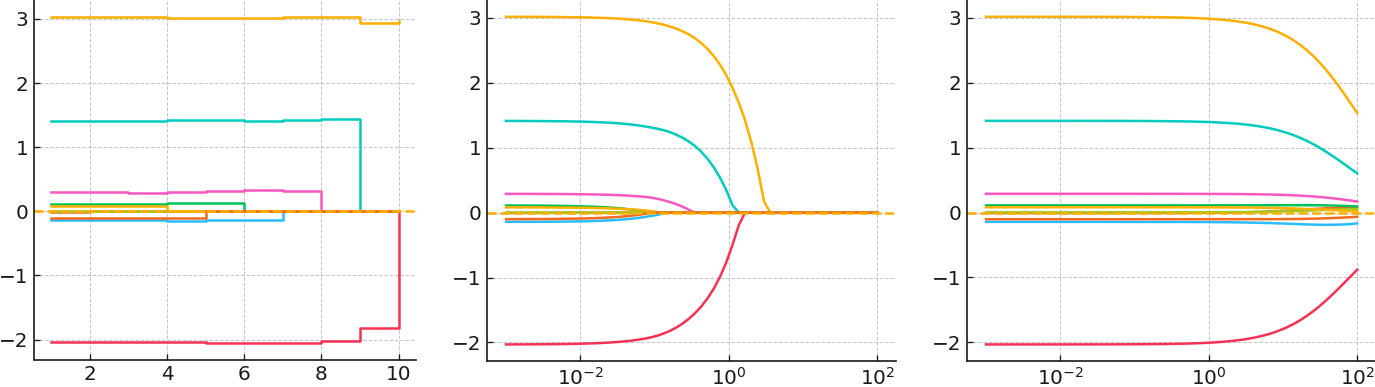
\includegraphics[width=0.98\columnwidth]{images/regularization_path_trim.png}
\end{center}
\begin{center}
    \textbf{Unit Balls of $\ell_p$ Norms in $\mathbb{R}^2$ for Varying $p$:}
    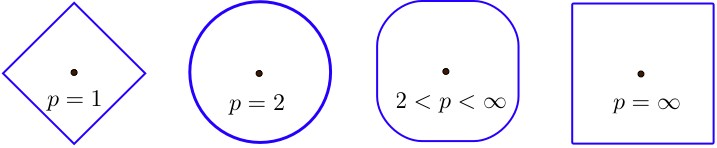
\includegraphics[width=0.9\columnwidth]{images/unit_balls.jpg}
\end{center}

\subsection{Hyperparameter Tuning}
\begin{itemize}
    \item \textbf{K-Fold Cross-Validation:}
\end{itemize}
    \input{subjects/model_selection}
    \section{Unsupervised Learning}

\subsection{Clustering}
\subsubsection{K-Means}
\begin{itemize}
    \item \textbf{Goal}: Partition $m$ samples into $k$ disjoint clusters
          so that points are \emph{as close as possible} to their
          respective cluster centroid.
    \item \textbf{Objective:} Minimize $\sum_j \sum_{x \in C_j} \|x - \mu_j\|^2$ \\
    (sum of squared distances to centroids).
    \item \textbf{Optimal clustering is NP-hard:} Cannot be solved exactly in polynomial time; K-Means is a heuristic that finds a local minimum.
\end{itemize}

%--------------------------- K-Means algorithm box ------------------------
\textbf{K-Means Algorithm (Lloyd's)}
\noindent
\fbox{\begin{minipage}{0.98\linewidth}
        \begin{algorithmic}
            \STATE \textbf{Input:} $X=\{x_1,\ldots,x_m\}\subset\mathbb{R}^{d}$, $k\in\mathbb{N}_{+}$
            \STATE Randomly choose initial centroids
                   $\mu_1,\ldots,\mu_k$
            \REPEAT
                \STATE \textbf{(Assignment)}\\
                       $C_j \leftarrow
                       \bigl\{x_i \;\big|\;
                             j
                             =\arg\min_{n}
                               \|x_i-\mu_n\|_2^{2}\bigr\}
                       \quad\forall j$
                \STATE \textbf{(Update)}\;
                       $\displaystyle
                       \mu_j \leftarrow
                       \frac{1}{|C_j|}\sum_{x \in C_j} x
                       \quad\forall j$
            \UNTIL{centroids unchanged \textbf{or}
                   assignments no longer move points}
            \STATE \textbf{Return:} clusters $C_1,\ldots,C_k$
        \end{algorithmic}
    \end{minipage}}

\begin{itemize}
    \item \textbf{Convergence}: Guaranteed to terminate in
          $\mathcal{O}(m)$ iterations, each strictly reducing $G$,
          but only to a \emph{local} minimum.
    \item \textbf{Sensitivity}: Result depends heavily on
          initial centroids;
    \item \textbf{Robustness}: Use \emph{multiple random restarts} for better results.
    \item \textbf{Bias-variance trade-off}: Higher $k$ reduces bias, increases variance.
\end{itemize}

%------------------------------------------------------------
\subsubsection{Spectral Clustering}
\revisit
\begin{itemize}
    \item \textbf{Goal}: Detect clusters based on the \emph{connectivity structure}
          of the data rather than purely geometric proximity.
    \item \textbf{Affinity graph}: Build a weighted, undirected graph
          on samples $X=\{x_1,\dots,x_m\}\subset \mathbb{R}^{d}$.
          For a bandwidth hyperparameter $\varepsilon>0$,
          \[
              A_{ij} \;=\;
              \exp\!\Bigl(-\tfrac{\|x_i-x_j\|_2^{2}}{\varepsilon}\Bigr)
              \quad(\text{often sparsified / $k$-NN}).
          \]
          $A\in\mathbb{R}^{m\times m}$ is the \emph{affinity matrix}.
    \item \textbf{Graph Laplacian (unnormalised)}:
          \[
              D \;=\; \operatorname{diag}\!\Bigl(\sum_{j}A_{ij}\Bigr),
              \quad
              L \;=\; D - A .
          \]
          (A normalised version $L_{\text{sym}}=D^{-1/2}LD^{-1/2}$ is common as well.)
    \item \textbf{Key spectral fact}:
          Number of connected components equals the multiplicity
          of eigenvalue $0$ of $L$ (spectral graph theory).
\end{itemize}

%--------------------- Spectral clustering algorithm box ------------------
\textbf{Spectral Clustering Algorithm (simplified)}
\noindent
\fbox{\begin{minipage}{0.98\linewidth}
        \begin{algorithmic}
            \STATE \textbf{Input:} data $X$, bandwidth $\varepsilon>0$, desired clusters $k$
            \STATE Build affinity matrix
                   $\displaystyle A_{ij}=\exp\!\bigl(-\|x_i-x_j\|_2^{2}/\varepsilon\bigr)$
            \STATE Compute degree matrix $D=\mathrm{diag}\!\bigl(\sum_j A_{ij}\bigr)$
            \STATE Form unnormalised Laplacian $L=D-A$
            \STATE Compute $k$ eigenvectors
                   $u_1,\dots,u_k$ of $L$ with \emph{smallest} eigenvalues
            \STATE Stack $U=[u_1,\dots,u_k]\in\mathbb{R}^{m\times k}$ ~(\(i\)-th row~$\to$~embedding of $x_i$)
            \STATE Apply K-Means to the rows of $U$ to obtain clusters $C_1,\dots,C_k$
            \STATE \textbf{Return:} $C_1,\dots,C_k$
        \end{algorithmic}
    \end{minipage}}

\begin{itemize}
    \item \textbf{No random initialisation} of centroids (randomness only from graph sparsification or K-Means post-step).
    \item \textbf{Hyperparameters}: bandwidth $\varepsilon$ and affinity type
          (heat kernel, $k$-NN graph, etc.).
    \item \textbf{Choosing $k$}: count eigenvalues of $L$ (or $L_{\text{sym}}$)
          that are \emph{close to zero} (eigengap heuristic).
    \item \textbf{Properties}:
          \begin{itemize}
              \item Captures \emph{non-convex} or \emph{manifold} clusters.
              \item More robust to noise than naïve connectivity methods.
              \item $\varepsilon$ acts as a bias–variance knob
                    (large $\varepsilon$~$\Rightarrow$ smoother, fewer clusters).
          \end{itemize}
\end{itemize}
%------------------------------------------------------------


\subsubsection{DBSCAN}
Density-based clustering that groups together points that are close to each other.

\subsubsection{Agglomerative Clustering}
Hierarchical clustering that merges clusters based on distance.

\begin{center}
    \textbf{KMeans vs. Spectral Clustering vs. DBSCAN}
    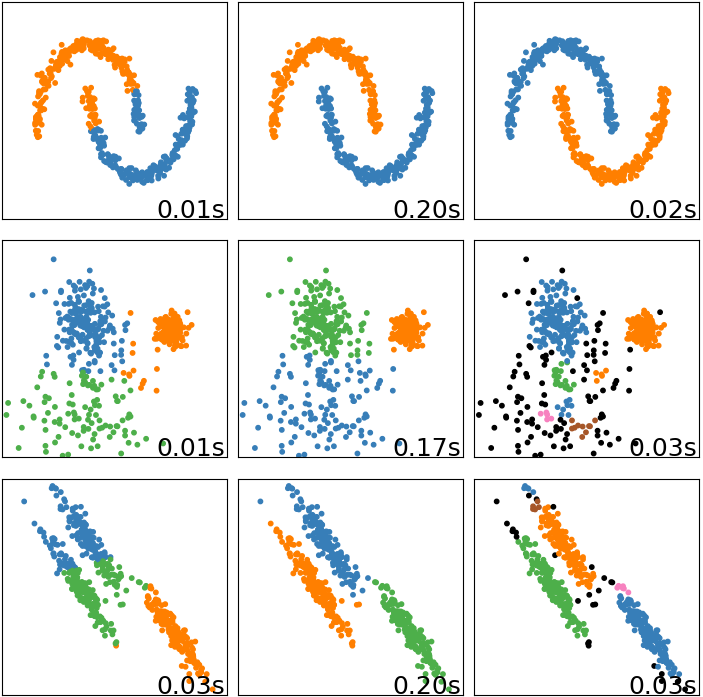
\includegraphics[width=0.9\columnwidth]{images/clustering_algos_3x3.png}
\end{center}

\subsection{Dimensionality Reduction}
\subsubsection{PCA (Principal Component Analysis)}
\begin{itemize}
    \item \textbf{Goal:} Find $k$ orthogonal directions (principal components) capturing maximal variance.
    \item \textbf{Formulation:} $W \in \mathbb{R}^{k \times d}$, $WW^T = I_k$
    \item \textbf{Optimization:} $w^* = \arg\max_{\{v_1,\ldots,v_k\}} \sum_{j=1}^k \mathrm{Var}(v_j^T X)$
    \item \textbf{Covariance Matrix:} $\Sigma = \frac{1}{m} \sum_{i=1}^m (x_i - \bar{x})(x_i - \bar{x})^T$
    \item \textbf{Principal Components:} Top $k$ eigenvectors of $\Sigma$ (correspond to largest eigenvalues)
    \item \textbf{Projection:} $x \mapsto W^T(x - \bar{x})$
    \item \textbf{Properties:} $\|x - v\|_2 \geq \|x - Px\|_2$ for $v \notin \mathrm{span}(u_1,\ldots,u_k)$
    \item \textbf{Explained Variance:} $\lambda_j$ is variance explained by $u_j$; $\sum_j \lambda_j$ is total variance.
\end{itemize}

\textbf{PCA Algorithm (Covariance-based)}
\noindent
\fbox{\begin{minipage}{0.98\linewidth}
        \begin{algorithmic}
            \STATE \textbf{Input:} $X \in \mathbb{R}^{m \times d}$ \quad \textit{(design matrix with $m$ samples, $d$ features)}
            \STATE Compute empirical mean: $\bar{x} \leftarrow \frac{1}{m} \sum_{i=1}^m x_i$
            \STATE Center the data: $Z \leftarrow X - \mathbf{1}\bar{x}^\top$
            \STATE Compute covariance matrix: $\Sigma \leftarrow \frac{1}{m} Z^\top Z$
            \STATE Eigen-decompose $\Sigma$; keep top $k$ eigenvectors $u_1,\ldots,u_k$
            \STATE \textbf{Return:} $u_1,\ldots,u_k$ \quad (principal component directions)
        \end{algorithmic}
    \end{minipage}}
\textit{Vectors $u_1,\ldots,u_k$ are orthonormal and maximise retained variance.}

    \section{Gradient Based Learning}

\textbf{Basic Idea} use an iterative optimization algorithm to minimize a loss function by updating parameters in the opposite direction of the gradient.

\subsection{Sub-gradient Concepts}
\begin{itemize}
    \item \textbf{Sub-gradient:} $v$ is a sub-gradient of $f$ at $w$ if $f(u) \geq f(w) + \langle v, u-w \rangle$ for all $u$.
    \item \textbf{Sub-differential:} $\partial f(w)$ is the set of all sub-gradients of $f$ at $w$.
    \item \textbf{Convexity:} $f$ is convex if $f(tv + (1-t)u) \leq t f(v) + (1-t)f(u)$ for $t \in [0,1]$.
    \item \textbf{Examples:} Halfspace, norm, sum of convex functions.
    \item \textbf{Directional derivative:} $f(y) \geq f(x) + \langle \nabla f(x), y-x \rangle$ for differentiable $f$.
\end{itemize}

\subsection{Backtracking Line Search Algorithm}
\noindent
\fbox{\begin{minipage}{0.98\linewidth}
        \begin{algorithmic}
            \STATE Initialize: $\eta = 1$
            \WHILE{$f(x) + \alpha \eta \langle \nabla f(x), \Delta x \rangle < f(x + \eta \Delta x)$}
            \STATE $\eta \leftarrow \beta \eta$ \hspace{1em} ($\beta \in (0,1)$)
            \ENDWHILE
            \STATE Return $\eta$
        \end{algorithmic}
    \end{minipage}}

\subsection{Sub-gradient Descent Algorithm}
\noindent
\fbox{\begin{minipage}{0.98\linewidth}
        \begin{algorithmic}
            \STATE Initialize: $w^{(1)} = 0$
            \FOR{$t = 1, \ldots, T$}
            \STATE Choose $v_t \in \partial f(w^{(t)})$
            \STATE $w^{(t+1)} \leftarrow w^{(t)} - \eta_t v_t$
            \ENDFOR
            \STATE Return $\bar{w} = \frac{1}{T} \sum_{t=1}^T w^{(t)}$
        \end{algorithmic}
    \end{minipage}}

\subsection{Stochastic Gradient Descent (SGD) Algorithm}
\noindent
\fbox{\begin{minipage}{0.98\linewidth}
        \begin{algorithmic}
            \STATE Initialize: $w^{(1)} = 0$
            \FOR{$t = 1, \ldots, T$}
            \STATE Choose $(x, y) \sim \mathcal{D}$
            \STATE Choose $v_t \in \partial \ell(w^{(t)}, (x, y))$
            \STATE $w^{(t+1)} \leftarrow w^{(t)} - \eta_t v_t$
            \ENDFOR
            \STATE Return $\bar{w} = \frac{1}{T} \sum_{t=1}^T w^{(t)}$
        \end{algorithmic}
    \end{minipage}}

    \section{Neural Networks}

\subsection{Backpropagation}
"Backpropagation is the algorithm for determining how a single training example would like to nudge the weights and biases (Gradient-based update), not just in terms of whether they should increase or decrease, but also in terms of the relative proportions that would cause the most rapid decrease in the cost function (Gradient direction). A true gradient descent step would involve computing these adjustments for all tens of thousands of training examples and averaging the resulting gradients. However, this is computationally expensive, so instead, the training data is randomly subdivided into mini-batches, and each gradient descent step is computed with respect to one mini-batch at a time. By repeatedly going through all of the mini-batches (Epoch) and updating the weights accordingly, the network gradually converges toward a local minimum of the cost function. In doing so, the network ends up performing very well on the training examples."


\textbf{Useful Terms:}
\begin{itemize}
    \item \textbf{Mini-batch:} A small subset of the training data used to compute the gradient for a single update step.
    \item \textbf{Batch Size:} The number of training examples in a mini-batch (hyperparameter).
    \item \textbf{Epoch:} One complete pass through the entire training dataset (via all mini-batches).
    \item \textbf{Dropout (rate):} A regularization technique where a fraction of neurons are randomly set to zero during a batch training to prevent overfitting. The rate is an hyperparameter (usually 50\%).
\end{itemize}

\begin{center}
    \textbf{Training Pipeline:}

    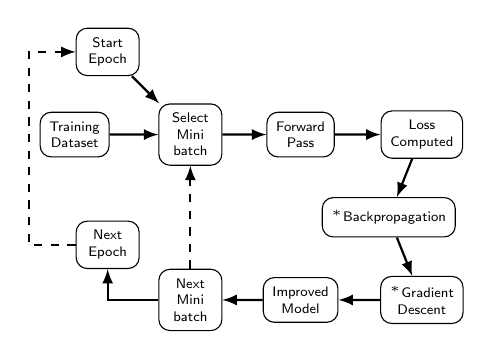
\begin{tikzpicture}[scale=0.7,
        every node/.style={draw, rounded corners, align=center, font=\tiny,
                minimum width=0.8cm, minimum height=0.5cm},
        arrow/.style={-{latex}, thick},
        dloop/.style={-{latex}, thick, dashed}
        ]

        % ---------------- Main pipeline ----------------
        \node (dataset)  at (-2.6,  1.5) {Training\\Dataset};
        \node (batch)    at ( -0.5,1.5) {Select\\Mini\\batch};
        \node (forward)  at ( 1.5,1.5) {Forward\\Pass};
        \node (loss)     at ( 3.7,1.5) {Loss\\Computed};
        \node (backprop) at ( 3.1,0)   {$^*$Backpropagation};
        \node (update)   at ( 3.7,-1.5){$^*$Gradient\\Descent};
        \node (improved) at ( 1.5,-1.5){Improved\\Model};

        % ---------------- Loop-control nodes -----------
        \node (nextbatch) at (-0.5,-1.5) {Next\\Mini\\batch};
        \node (epoch)     at (-2, 3)    {Start\\Epoch};
        \node (nextepoch) at (-2,-0.5)  {Next\\Epoch};

        % ---------------- Straight arrows --------------
        \draw[arrow] (dataset)  -- (batch);
        \draw[arrow] (batch)    -- (forward);
        \draw[arrow] (forward)  -- (loss);
        \draw[arrow] (loss)     -- (backprop);
        \draw[arrow] (backprop) -- (update);
        \draw[arrow] (update)   -- (improved);
        \draw[arrow] (improved) -- (nextbatch);

        % ---------------- Mini-batch loop (dashed) -----
        \draw[dloop] (nextbatch.north) -- (batch.south);

        % ---------------- Epoch loop (dashed) ----------
        \draw[arrow] (nextbatch.west) -- ++(-0.50,0) -| (nextepoch.south);      % end of last mini-batch
        \draw[dloop] (nextepoch.west) -- ++(-0.85,0) |- (epoch.west);
        \draw[arrow] (epoch) -- (batch);              % new epoch begins

    \end{tikzpicture}

    \textit{$^*$Backpropagation computes gradients; a gradient-based optimiser applies them over many mini-batches and epochs.}

\end{center}


\subsection{FNNs (Feedforward Neural Networks)}

\subsection{CNNs (Convolutional Neural Networks)}

\subsection{RNNs (Recurrent Neural Networks)}

RNNs process sequential data, using previous steps to inform current predictions. Useful for text, audio, etc. and supports one/many-to-one/many sequence I/O patterns (e.g image $\to$ description is one-to-many).

$h_t = \tanh(U h_{t-1} + V x_t)$

\subsubsection{Basic RNN}
\textbf{Diagrams notation:}
\begin{center}
    % https://colah.github.io/posts/2015-08-Understanding-LSTMs
    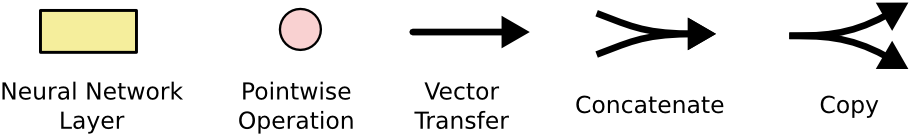
\includegraphics[width=0.98\columnwidth]{images/rnn_notations.png}
\end{center}

\textbf{RNN Cell:}
\begin{center}
    % https://colah.github.io/posts/2015-08-Understanding-LSTMs
    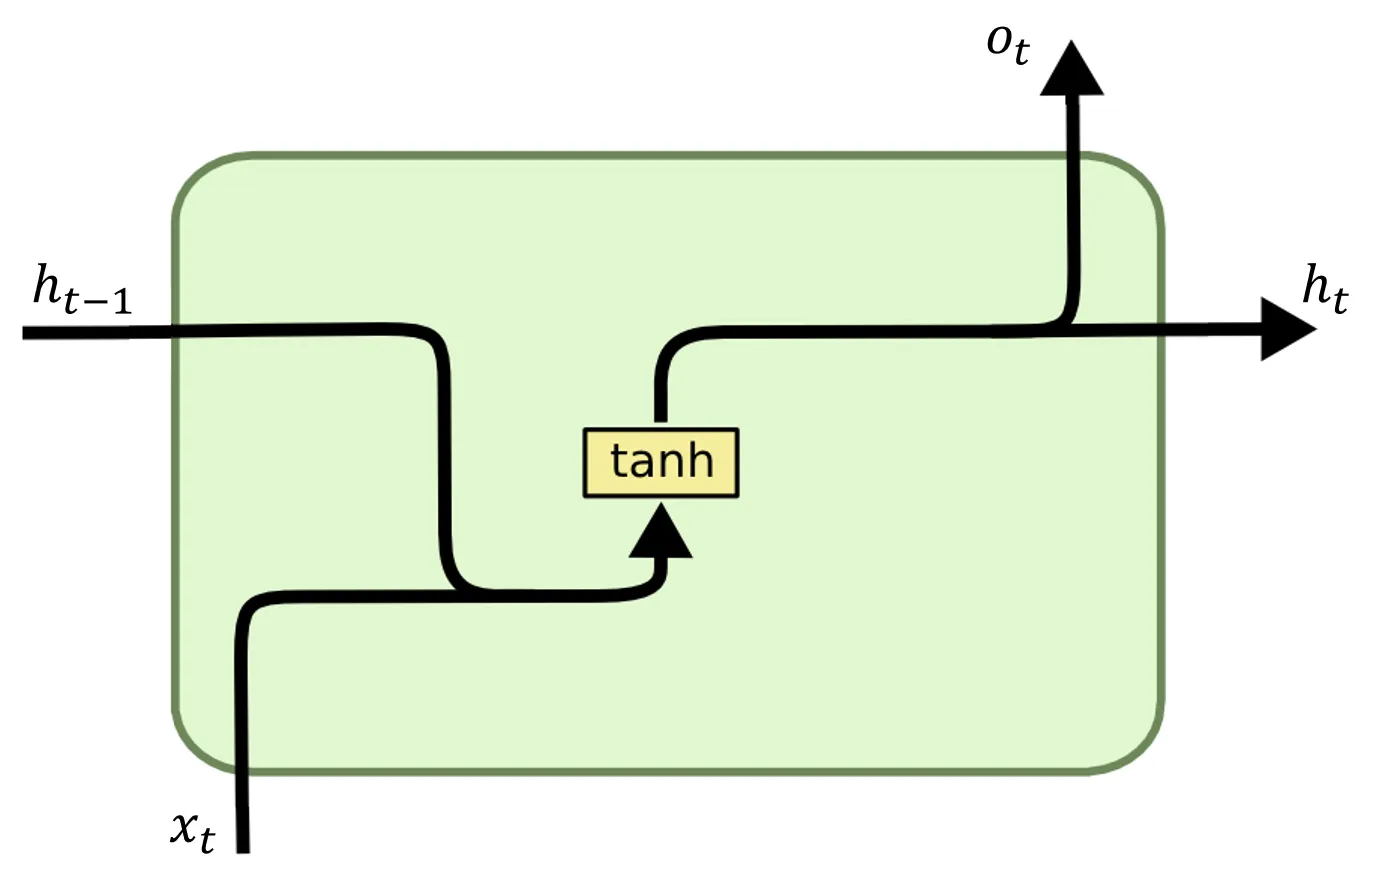
\includegraphics[width=0.98\columnwidth]{images/rnn_cell.png}
\end{center}

\subsubsection{Long Short-Term Memory (LSTM)}

LSTMs are a type of RNN designed to remember information for long periods, addressing the vanishing gradient problem. They achieve this through a cell state ($C_t$) and three gates: input ($i_t$), forget ($f_t$), and output ($o_t$).

\begin{center}
    % https://colah.github.io/posts/2015-08-Understanding-LSTMs
    % LSTM Cell Diagram with included title
    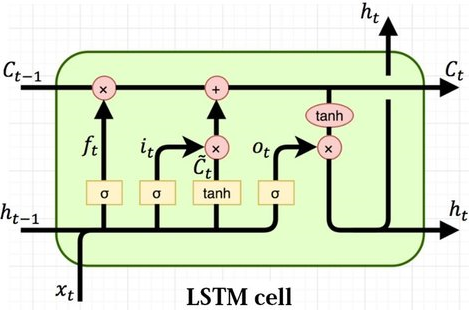
\includegraphics[width=0.98\columnwidth]{images/lstm_cell_trim.png}
\end{center}

\text{Where:}
\begin{itemize}
    \item $i_t = \sigma(x_t U^i + h_{t-1} W^i) \quad$ Input gate, controls how much of the input to let through.
    \item $f_t = \sigma(x_t U^f + h_{t-1} W^f) \quad$ Forget gate, controls how much of the previous cell state to keep.
    \item $o_t = \sigma(x_t U^o + h_{t-1} W^o) \quad$ Output gate, controls how much of the cell state to output.
    \item $\tilde{c}_t = \tanh(x_t U^g + h_{t-1} W^g) \quad$ Candidate cell state, potential new information to add to the cell state.
    \item $c_t = \sigma(f_t * C_{t-1} + i_t * \tilde{C}_t) \quad$ Cell state, memory of the LSTM.
    \item $h_t = \tanh(C_t) * o_t \quad$ Hidden state, output of the LSTM at time $t$.
\end{itemize}

\textbf{LSTM Chain:}
\begin{center}
    % https://colah.github.io/posts/2015-08-Understanding-LSTMs
    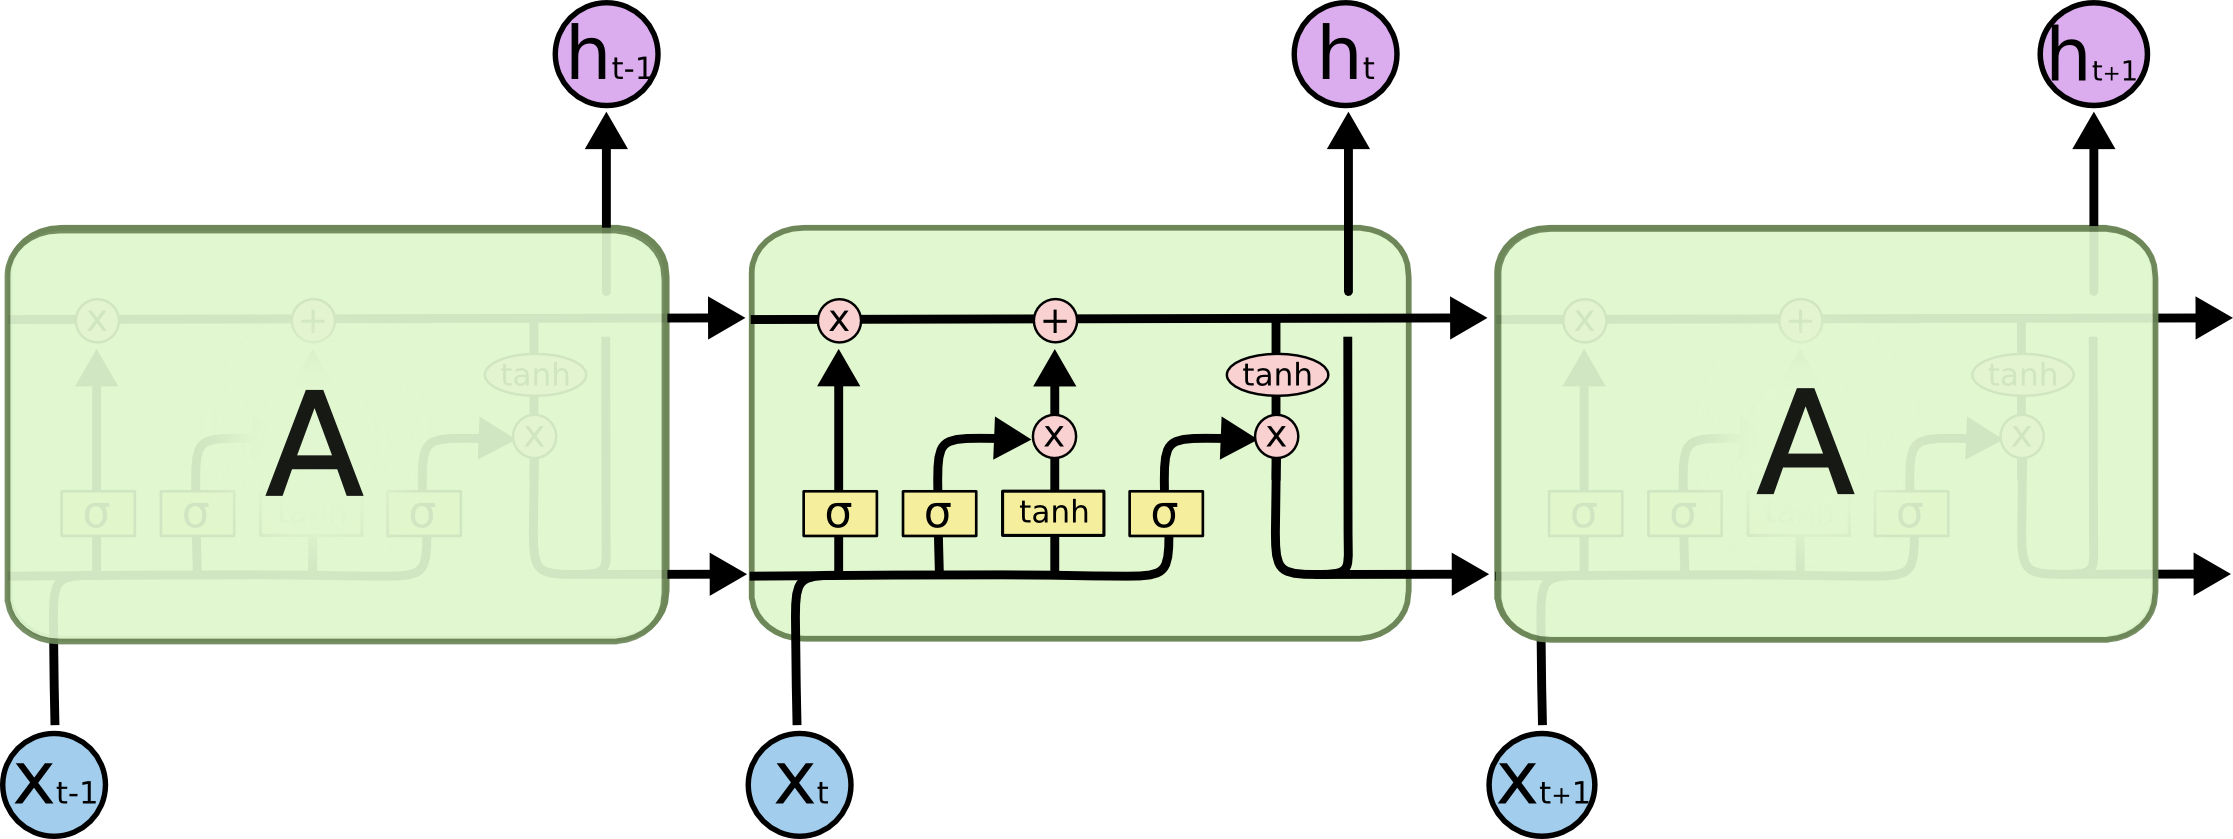
\includegraphics[width=0.98\columnwidth]{images/lstm-chain.png}
\end{center}

\subsubsection{RNNs vs. CNNs}
\begin{center}
    \resizebox{\columnwidth}{!}{
    \begin{tabular}{lcc}
        \hline
        \textbf{Property}                    & \textbf{RNN}     & \textbf{CNN} \\
        \hline
        Long-range mechanism                 & Gating/Attention & Pooling      \\
        Sequential                           & $+$              & $-$          \\
        Parallelizable                       & $-$              & $+$          \\
        Compute time for $n$ tokens          & $O(n\cdot L)$    & $O(L)$       \\
        Layers required for the $n$-th token & $1$              & $\log n$     \\
        \hline
    \end{tabular}
    }
\end{center}
\end{multicols*}

\end{document}